\chapter{Tutorial}
\label{Tutorial}
\typeout{$Id$}

\section{Creating a Template Bundle}

To create information sheets for your game elements, you will need to
create templates\footnote{A pre-built template bundle for
\textit{Advanced Dungeond and Dragons}, dnd.rpgtmpl, is included, so if
you play using the \textit{Advanced Dungeond and Dragons} system, you
are all set to go.}.

\begin{figure}[hbpt] 
\begin{centering}
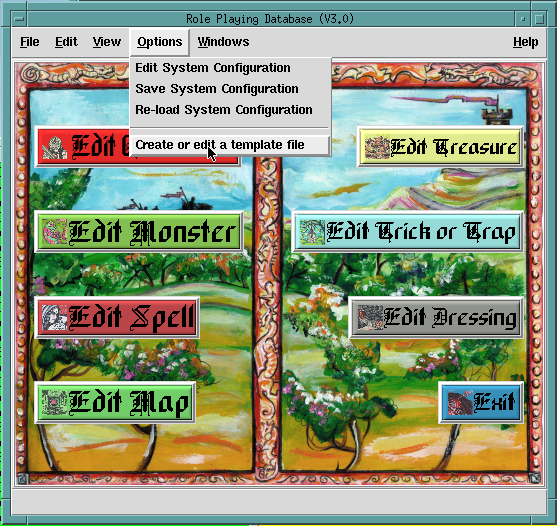
\includegraphics[width=5in]{OptionMenu.png} 
\caption{Selecting ``Create or edit a template file''} 
\label{fig:createoredittemplatemenu} 
\end{centering}
\end{figure} 
\begin{figure}[hbpt] 
\begin{centering}
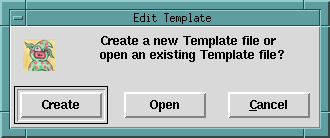
\includegraphics{CreateOrEditTemplateDialog.png} 
\caption{The Create Or Edit Template Dialog}
\label{fig:createoredittemplate} 
\end{centering}
\end{figure} 
\begin{figure}[hbpt]
\begin{centering}
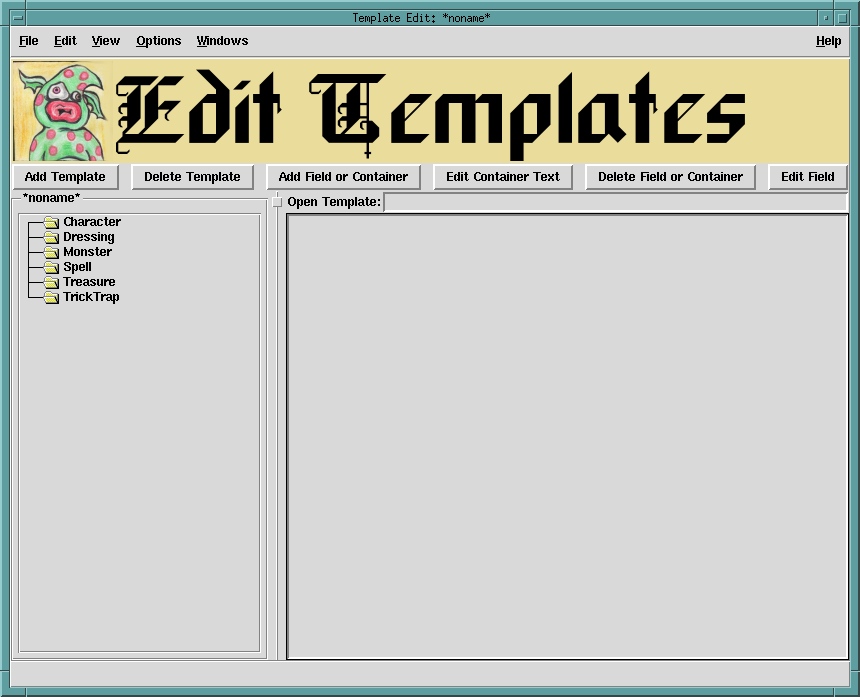
\includegraphics[width=5in]{EmptyTemplateEditor.png}
\caption{Empty Template Editor Window}
\label{fig:emptytemplate}
\end{centering}
\end{figure}
\begin{figure}[hbpt]
\begin{centering}
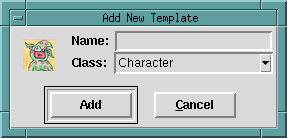
\includegraphics{AddNewTemplate.png}
\caption{Add New Template Dialog Box}
\label{fig:addnewtemplate}
\end{centering}
\end{figure}
\begin{figure}[hbpt]
\begin{centering}
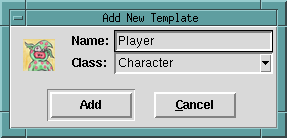
\includegraphics{AddNewTemplatePlayer.png}
\caption{Add New Template Dialog Box, with ``Player'' filled in}
\label{fig:addnewtemplateplayer}
\end{centering}
\end{figure}
\begin{figure}[hbpt]
\begin{centering}
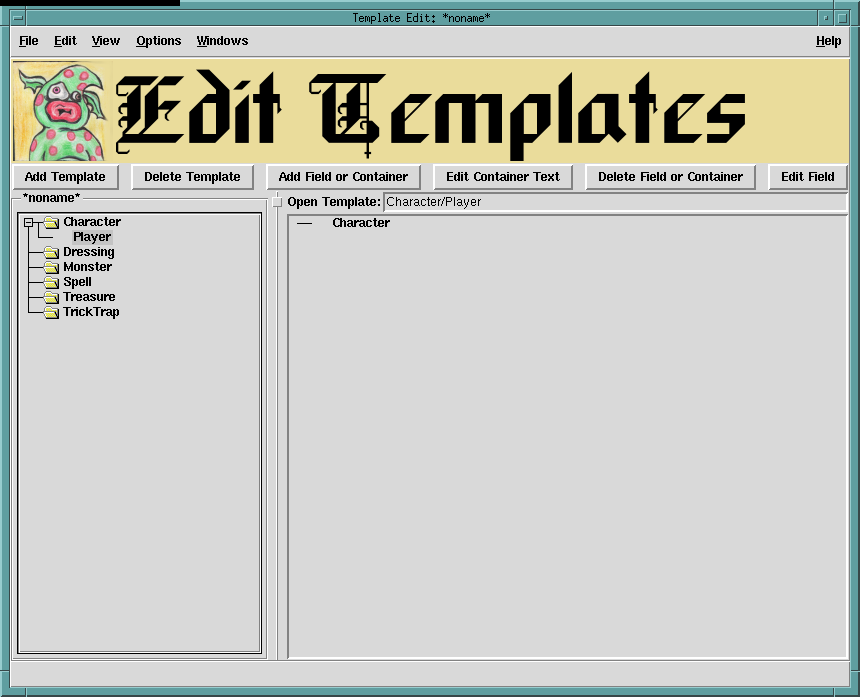
\includegraphics[width=5in]{PlayerTemplateEditor.png}
\caption{Template Editor, with empty ``Player'' template}
\label{fig:emptyplayertemplateeditor}
\end{centering}
\end{figure}
To create a template bundle, select ``Create or edit a template file''
from the Options menu, as shown in
Figure~\ref{fig:createoredittemplatemenu}.  This will display the dialog box
shown in Figure~\ref{fig:createoredittemplate}.  Select ``Create''.  An
empty template editor window, as shown in Figure~\ref{fig:emptytemplate}
will be opened up.  You can now start to create templates for your game
system.  We will create a simple Character class template.  First, click
on ``Add Template''.  This will open up the ``Add New Template'' dialog
box, as shown in Figure~\ref{fig:addnewtemplate}.  Type ``Player'' in
the name field, as shown in Figure~\ref{fig:addnewtemplateplayer}, and
click ``Add''.  This will create an entry under the ``Character'' folder
named ``Player''.  Double click on this entry now.  The template editor
will will now look like Figure~\ref{fig:emptyplayertemplateeditor}.

\subsection{Adding heading text to a container}

\begin{figure}[hbpt]
\begin{centering}
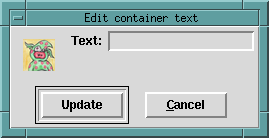
\includegraphics{EmptyEditContainerText.png}
\caption{Empty ``Edit Container Text'' dialog box}
\label{fig:editcontainertext}
\end{centering}
\end{figure}
\begin{figure}[hbpt]
\begin{centering}
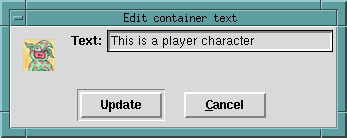
\includegraphics{EditContainerTextWithText.png}
\caption{``Edit Container Text'' dialog box with text added}
\label{fig:editcontainertextwithtext}
\end{centering}
\end{figure}
\begin{figure}[hbpt]
\begin{centering}
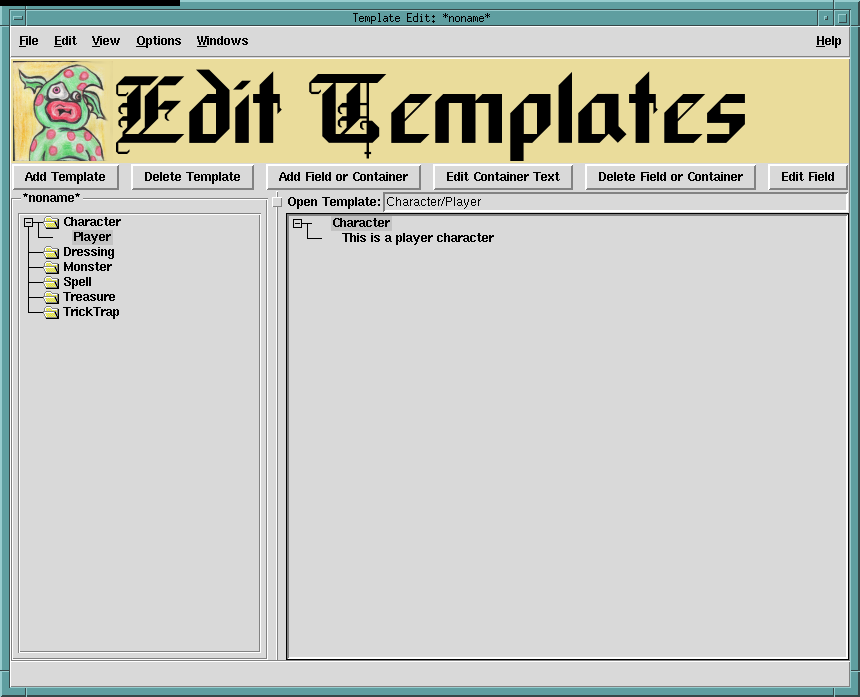
\includegraphics[width=5in]{PlayerTemplateEditorHeading.png}
\caption{Template Editor, with ``Player'' template, with a heading added}
\label{fig:playertemplateeditorwithheading}
\end{centering}
\end{figure}
At first, all that is in a sheet template is an empty toplevel
container, named for the class of sheet (Character) in this case.  The
first thing you will want to do is add a heading for this container.
Highlight the container name by clicking on it, then click the ``Edit
Continer Text'' button on the tool bar.  This will display the ``Edit
Container Text'' dialog box, as shown in
Figure~\ref{fig:editcontainertext}. Fill in the text field with ``This
is a player character''.  The dialog box will now look like
Figure~\ref{fig:editcontainertextwithtext}. Click ``Update''. The
template editor window will now look like
Figure~\ref{fig:playertemplateeditorwithheading}.

\subsection{Adding a field to a container}

\begin{figure}[hbpt]
\begin{centering}
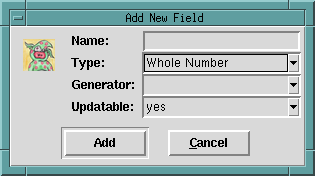
\includegraphics{AddNewFieldDialog.png}
\caption{``Add New Field'' dialog box}
\label{fig:addnewfield}
\end{centering}
\end{figure}
\begin{figure}[hbpt]
\begin{centering}
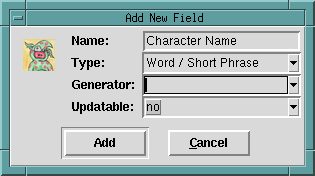
\includegraphics{AddNewFieldDialogWithField.png}
\caption{``Add New Field'' dialog box with field values filled in}
\label{fig:addnewfieldfilledin}
\end{centering}
\end{figure}
\begin{figure}[hbpt]
\begin{centering}
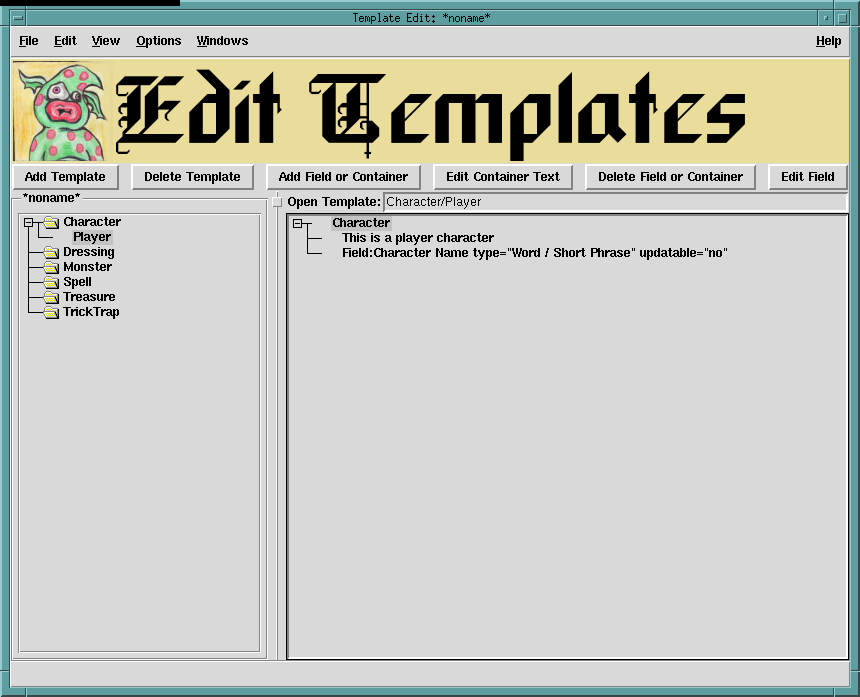
\includegraphics[width=5in]{PlayerTemplateEditorWithField.png}
\caption{Template Editor, with ``Player'' template, with a field added}
\label{fig:playertemplateeditorwithfield}
\end{centering}
\end{figure}
To add a field to the toplevel container, make sure the container name
is highlighter (click on the name to be sure), and click on the ``Add
Field or Container''.  This will display the ``Add New Field'' dialog
box, shown in Figure~\ref{fig:addnewfield}.  Fill in the ``Name'' field
with ``Character Name'', select ``Word / Short Phrase'' from the
``Type'' menu, and set ``Updatable'' to ``no''.  The dialog box should
now look like Figure~\ref{fig:addnewfieldfilledin}.  Click the ``Add''
button on the dialog box.  The template editor window should now look
like Figure~\ref{fig:playertemplateeditorwithfield}.

\subsection{Adding a container to a container}

\begin{figure}[hbpt]
\begin{centering}
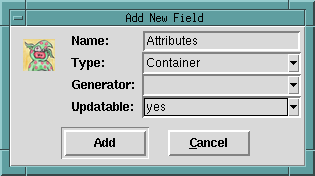
\includegraphics{AddNewFieldDialogWithContainer.png}
\caption{``Add New Field'' dialog box with container}
\label{fig:addnewcontainer}
\end{centering}
\end{figure}
\begin{figure}[hbpt]
\begin{centering}
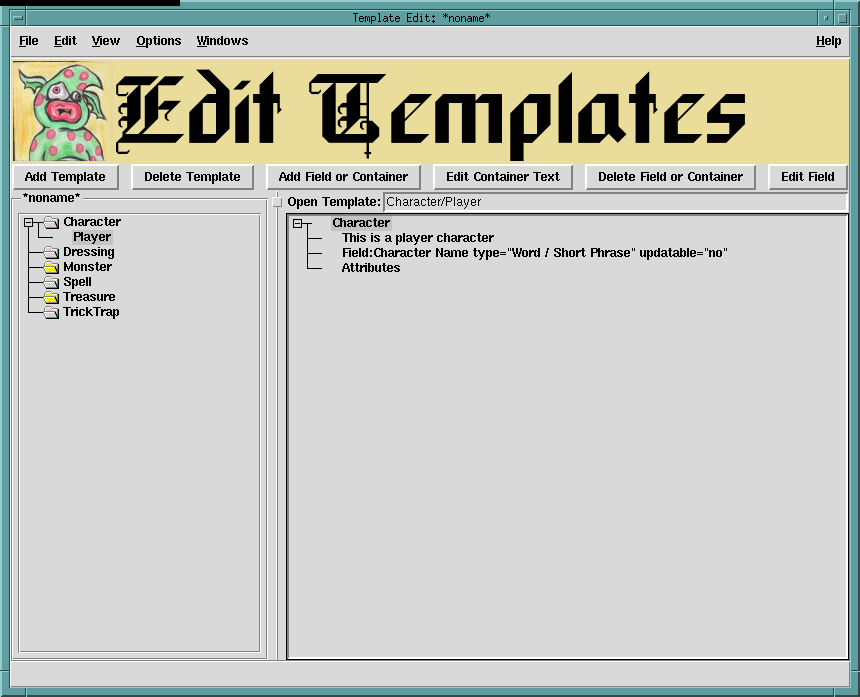
\includegraphics[width=5in]{PlayerTemplateEditorWithContainer.png}
\caption{Template Editor, with ``Player'' template, with a container added}
\label{fig:playertemplateeditorwithcontainer}
\end{centering}
\end{figure}
To add a container to the toplevel container, make sure the container name
is highlighter (click on the name to be sure), and click on the ``Add
Field or Container''.  This will display the ``Add New Field'' dialog
box, shown in Figure~\ref{fig:addnewfield}.  Fill in the ``Name'' field
with ``Attributes'', select ``Container'' from the
``Type'' menu, and set ``Updatable'' to ``yes''.  The dialog box should
now look like Figure~\ref{fig:addnewcontainer}.  Click the ``Add''
button on the dialog box.  The template editor window should now look
like Figure~\ref{fig:playertemplateeditorwithcontainer}.

\section{Creating a character sheet}

\begin{figure}[hbpt]
\begin{centering}
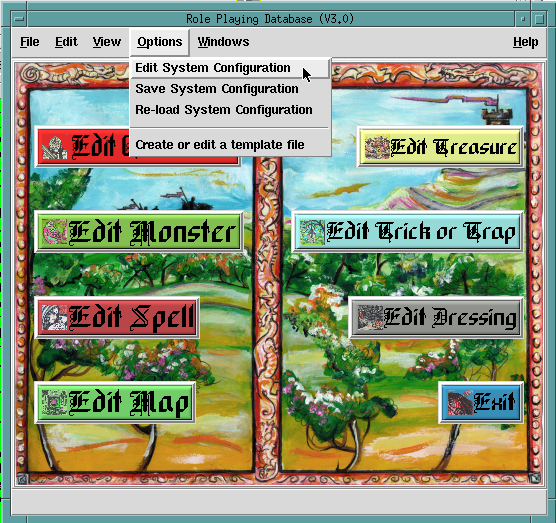
\includegraphics[width=5in]{OpenConfigurationEditor.png}
\caption{Selecting ``Edit System Configuration'' from the ``Options'' menu}
\label{fig:opensysconfedit}
\end{centering}
\end{figure}
To create a character sheet, we first need to be sure that there is an
available template bundle.  Go to the \verb=Options= menu and select
\verb=Edit System Configuration=, as shown in
Figure~\ref{fig:opensysconfedit}. Click on the file folder button to the
right of the ``Template File'' field and navigate to the location of the
\verb=dnd.rpgtmpl= file included with the \thesystem. Click ``Open'' on
the file select dialog and then ``OK'' on the configuration editor
window.  You might want then go to the \verb=Options= menu and select
\verb=Save System Configuration= to write out this configuration.

\begin{figure}[hbpt]  
\begin{centering}
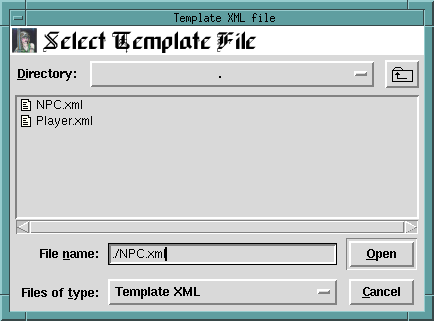
\includegraphics{SelectTemplateFile.png} 
\caption{The ``Select Template File'' dialog} 
\label{fig:selecttemplatefile} 
\end{centering}
\end{figure} 
\begin{figure}[hbpt] 
\begin{centering}
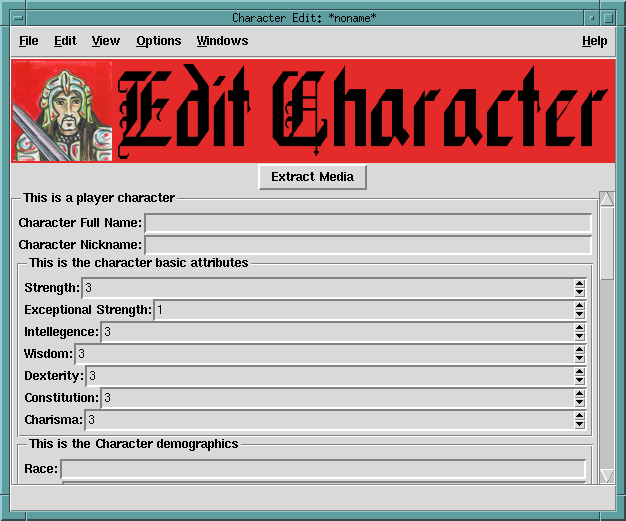
\includegraphics[width=5in]{EmptyPlayerCharacterSheet.png} 
\caption{An empty player character sheet} 
\label{fig:emptyplayercharacter}
\end{centering} 
\end{figure} 
Next, click on the \verb=Edit Character= button.  This will open the
``Open or Create Character'' dialog box, shown in
Figure~\ref{fig:opencreatechar}.  Click on the file folder button. 
This will open the ``Select Template File'' dialog, shown in
Figure~\ref{fig:selecttemplatefile}. Double click on ``Player.xml''. 
This will select the player template, rather than the default
non-player character (NPC) template.  Now click on the ``Create''
button on the ``Open or Create Character'' dialog box.  You should now
have an empty character sheet much like that shown in
Figure~\ref{fig:emptyplayercharacter}. You are now ready to create a
player character sheet!  The process is much like filling in a form.
Each piece of information is filled into a labeled space.  Numeric
values have small up and down arrows at the right end of the field and
you can either type in the numbers or use these arrows to increase or
decrease the value in the field.  Fields which take file names have a
folder button at the right end.  These buttons can be clicked on to
open a file browser to select the file\footnote{External files are
copied into the sheet bundle to allow for easy transport and sharing.}.
 Text areas will display a scroll bar once the amount of text grows to
be long enough to need it. The sheet is broken up into sections.  First
there is the character's full name and his or her nickname(s).  The
next section is the character's basic attributes: Strength,
Intellegence, Wisdom, Dexterity, Constitution, and Charisma.  Then
comes the character's demographics, which includes the characters race,
class, gender, age, and alignment.  Then the character's wealth and
health: gold pieces, hit points, experience points, and level.  Then
comes the extra detail, which includes a picture, a short bio, and a
full bio.  Finally there is information about the player, including the
player's name, address, phone number and E-Mail address.  Some of these
fields will be filled out with the help of your game master and some
fields will be filled in from dice rolls\footnote{The \thesystem\  does
not include a dice roll function, since it is expected that most
players would prefer to use their own dice or other source of random
numbers.}.

\section{Creating a map}


\begin{figure}[hbpt] 
\begin{centering}
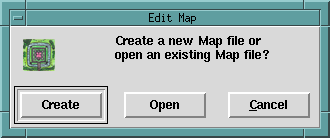
\includegraphics{CreateOrOpenMap.png} 
\caption{``Create or open a Map file'' dialog box} 
\label{fig:createoropenmap} 
\end{centering}
\end{figure} 
\begin{figure}[hbpt]
\begin{centering}
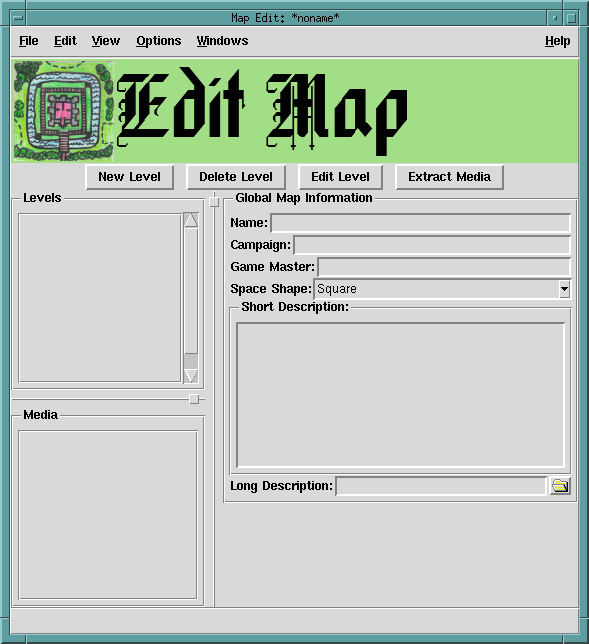
\includegraphics[width=5in]{EmptyMapEditorWindow.png}
\caption{Empty ``Edit Map'' window}
\label{fig:emptymapeditor}
\end{centering}
\end{figure}
\begin{figure}[hbpt]
\begin{centering}
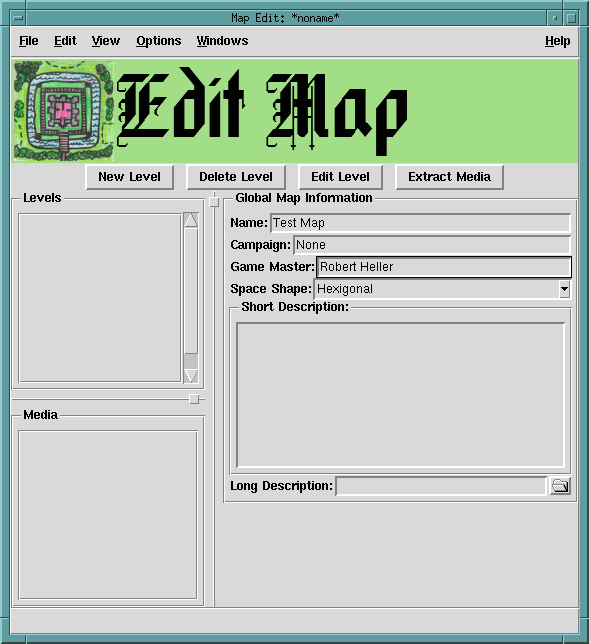
\includegraphics[width=5in]{TestMapEditorWindow1.png}
\caption{Test ``Edit Map'' window, after entering the basic map information}
\label{fig:testmapeditor1}
\end{centering}
\end{figure}
To create a map you need to click on the ``Edit Map'' button.  A dialog
box, shown in Figure~\ref{fig:createoropenmap}, will be displayed. 
Click the ``Create'' button.  You should now have an empty ``Edit Map''
window, as shown in Figure~\ref{fig:emptymapeditor}.  You can now fill
in the basic map information, which includes the Name (enter ``Test
Map''), the Campaign (enter ``None''), the Game Master (enter your
name), and the Space Shape (select ``Hexigonal'').  You can leave the
Short and Long Descriptions blank for now, but for a real map it is
probably a good idea to write a paragraph or two for the Short
Description, if only to remind you of what this map is for. The map
editor should now look something like Figure~\ref{fig:testmapeditor1}.

\subsection{Creating a new level}

\begin{figure}[hbpt] 
\begin{centering}
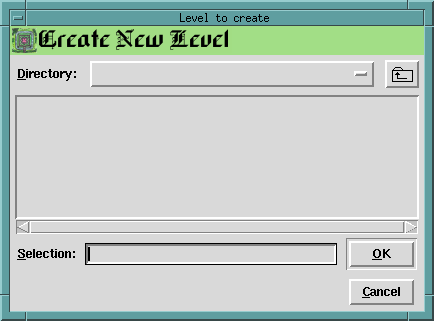
\includegraphics{CreateNewLevel.png} 
\caption{``Create New Level'' dialog box} 
\label{fig:createnewlevel} 
\end{centering}
\end{figure} 
\begin{figure}[hbpt]
\begin{centering}
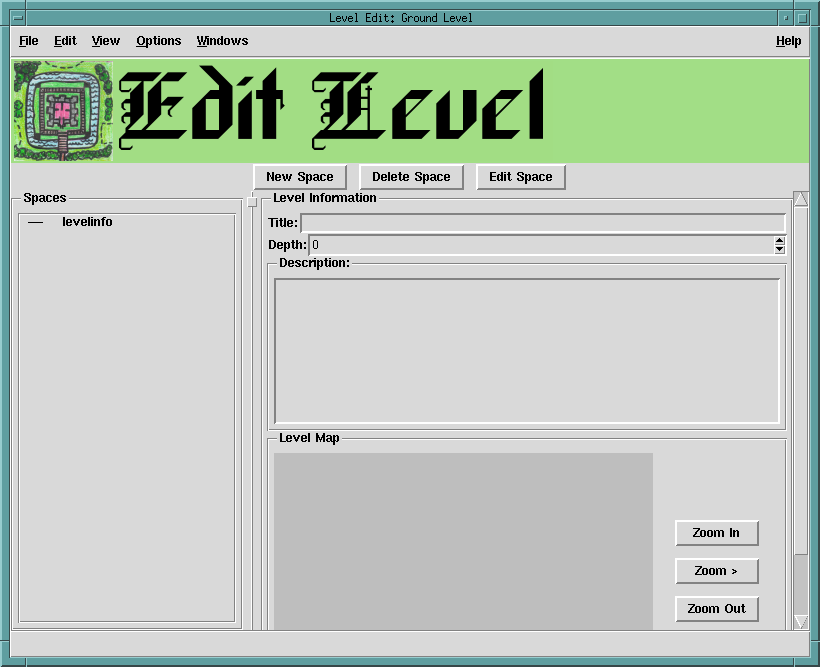
\includegraphics[width=5in]{EmptyLevelEditorWindow.png}
\caption{Empty ``Edit Level'' window}
\label{fig:emptyleveleditor}
\end{centering}
\end{figure}
\begin{figure}[hbpt]
\begin{centering}
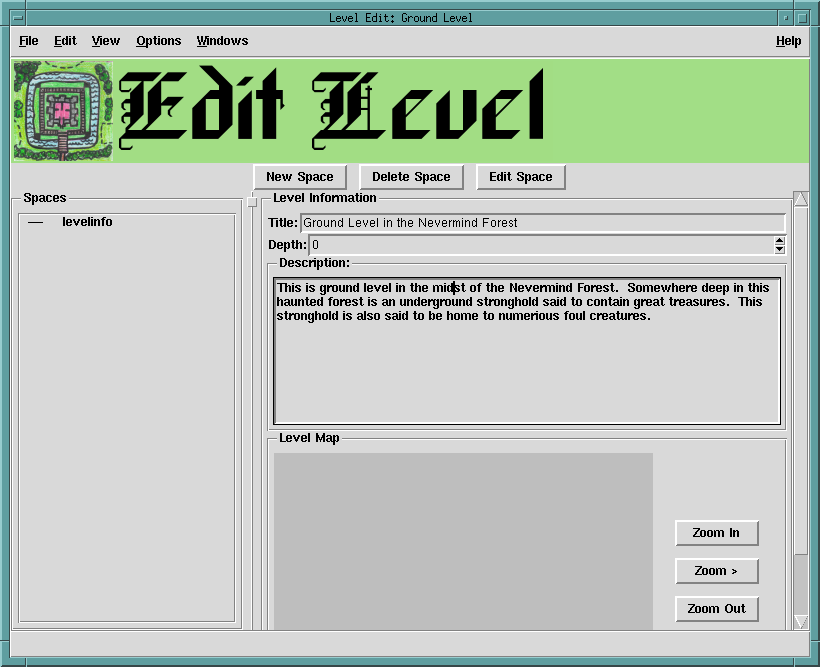
\includegraphics[width=5in]{ExampleLevelEditorWindow.png}
\caption{Example ``Edit Level'' window}
\label{fig:exampleleveleditor}
\end{centering}
\end{figure}
To create a new level, click the ``New Level'' button on the map editor
tool bar.  This will display the ``Create New Level'' dialog box, shown
in Figure~\ref{fig:createnewlevel}. Enter ``Ground Level'' in the
Selection entry and click ``Open'' twice.  You should now have an empty
``Edit Level'' window, as shown in Figure~\ref{fig:emptyleveleditor}. 
The level's basic information can be filled in.  The depth is the depth
below ground (when negative) or height above ground (when positive).  A
depth of zero is at ground level.  The title can be a short name for the
level and the description can be a longer description.  An filled in
example is shown in Figure~\ref{fig:exampleleveleditor}.

\subsection{Creating a space}

\begin{figure}[hbpt]
\begin{centering}
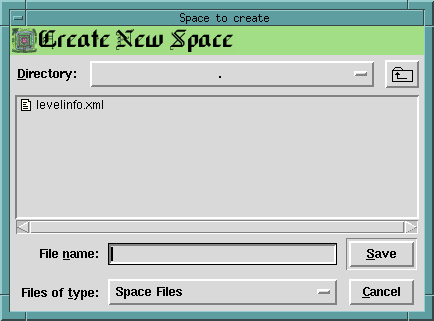
\includegraphics{CreateNewSpace.png}
\caption{``Create New Space'' dialog box}
\label{fig:createnewspace}
\end{centering}
\end{figure}
\begin{figure}[hbpt]
\begin{centering}
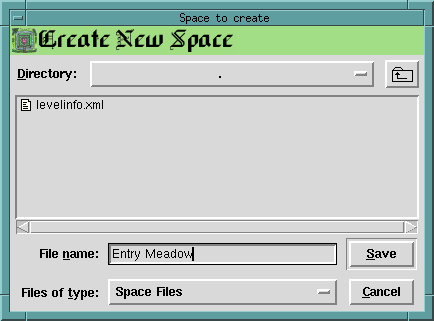
\includegraphics{CreateEntryMeadowSpace.png}
\caption{``Create New Space'' dialog box with ``Entry Meadow'' filled
in}
\label{fig:createentrymeadownewspace}
\end{centering}
\end{figure}
\begin{figure}[hbpt]
\begin{centering}
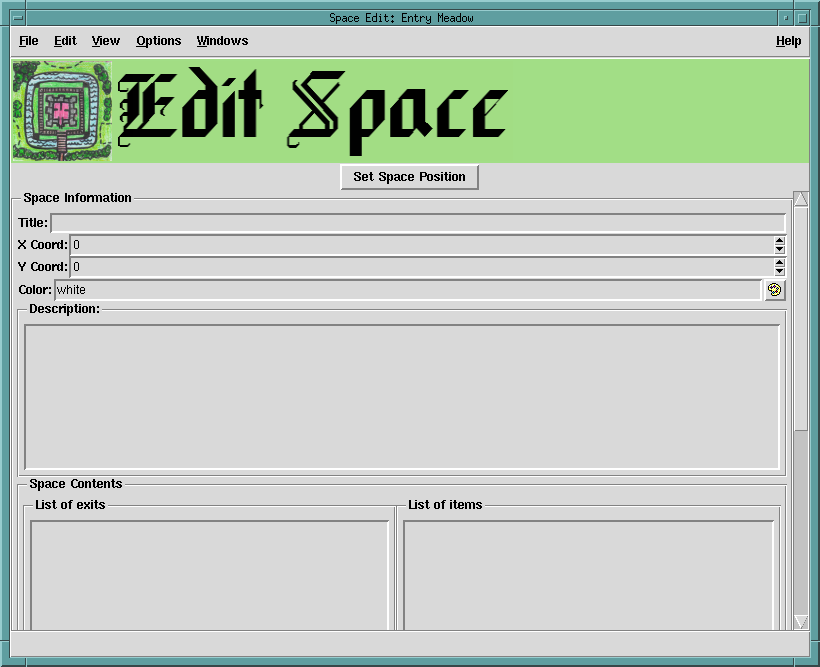
\includegraphics[width=5in]{NewEntryMeadowSpace.png}
\caption{Empty ``Space Editor'' window}
\label{fig:emptyspaceeditor}
\end{centering}
\end{figure}
\begin{figure}[hbpt]
\begin{centering}
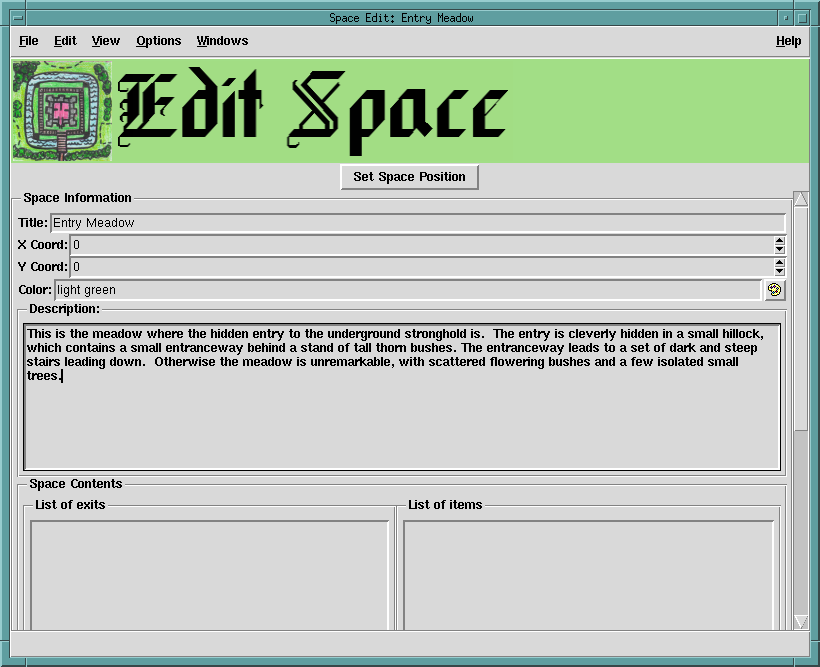
\includegraphics[width=5in]{EntryMeadowSpaceBasicInformation.png}
\caption{``Space Editor'' window with ``Entry Meadow'' information
filled in}
\label{fig:entrymeadowspaceeditor1}
\end{centering}
\end{figure}
\begin{figure}[hbpt]
\begin{centering}
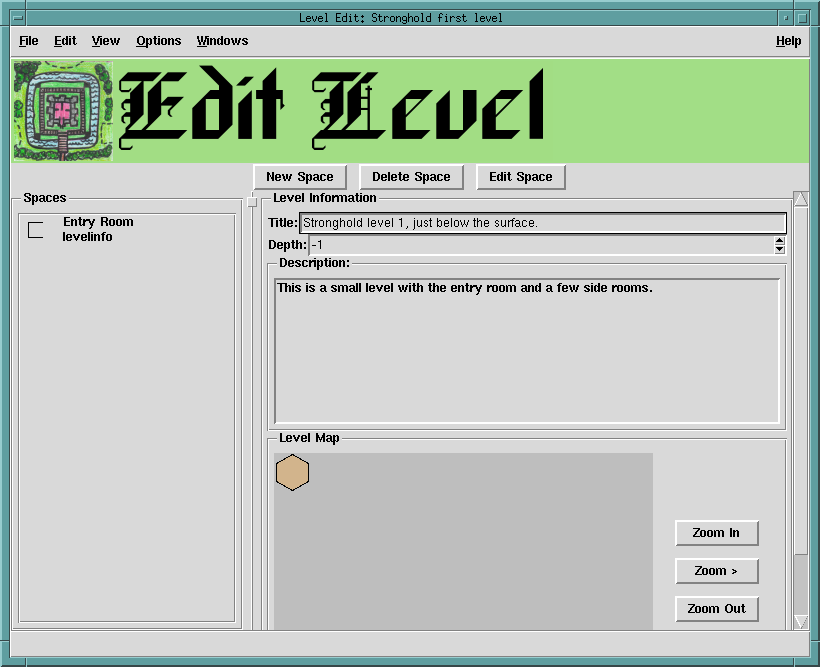
\includegraphics[width=5in]{StrongholdLevel1.png}
\caption{``Level Editor'' window ``Stronghold Level 1''}
\label{fig:strongholdl1}
\end{centering}
\end{figure}
\begin{figure}[hbpt]
\begin{centering}
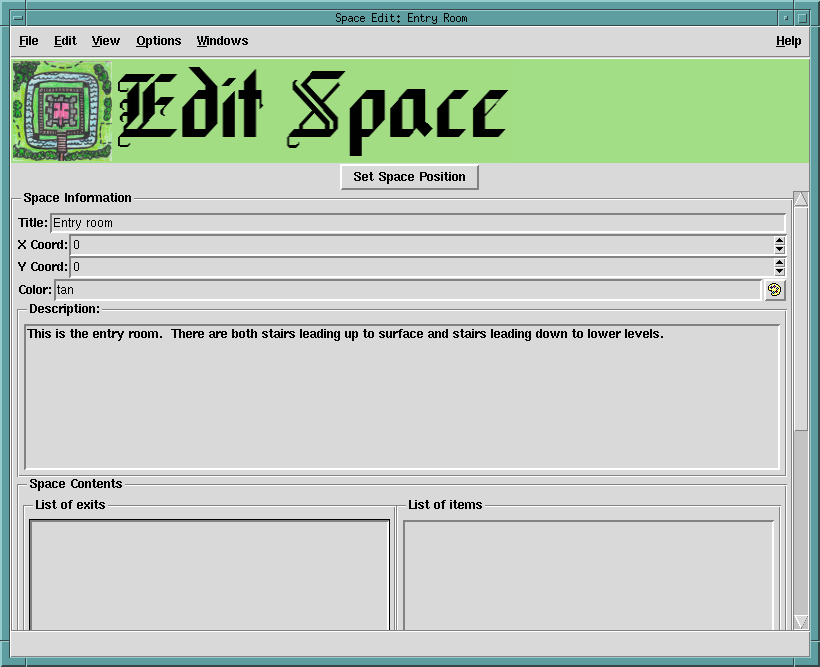
\includegraphics[width=5in]{EntryRoom.png}
\caption{``Space Editor'' window with ``Entry Room'' information
filled in}
\label{fig:entryroom}
\end{centering}
\end{figure}
To create a new space, click on the ``New Space'' button on the level
editor window.  This will display a ``Create New Space'' dialog box,
shown in Figure~\ref{fig:createnewspace}.  Fill in ``Entry Meadow'' as
the filename, as shown in Figure~\ref{fig:createentrymeadownewspace},
and click ``Create''.  This will open a new space editor window, as
shown in Figure~\ref{fig:emptyspaceeditor}.  You can now enter the
space's basic information as show in
Figure~\ref{fig:entrymeadowspaceeditor1}.  You should now save things,
by selecting the ``Save'' menu item on the ``File'' menu.  We will come
back to this space later.  For now, we need to create a space on a
different level in order to add the hidden stairs down to the
underground stronghold.  We will do this by creating a new level named
``Stronghold first level'', which will be at a depth of -1, then create
a space at location 0,0 on this level named ``Entry Room''. We now have
two additional windows, as shown in Figures~\ref{fig:strongholdl1} and
\ref{fig:entryroom}.

\subsubsection{Adding items and exits to a space}

\begin{figure}[hbpt]
\begin{centering}
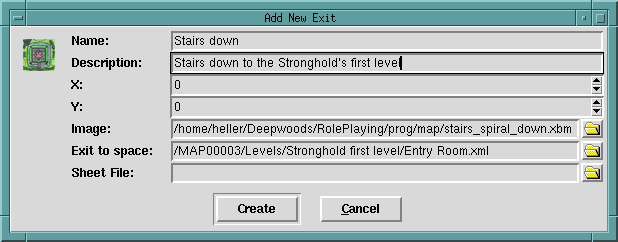
\includegraphics[width=5in]{CreatingStairsDown.png}
\caption{``Add New Edit'' dialog box, adding the entrance stairs}
\label{fig:addnewexit}
\end{centering}
\end{figure}
\begin{figure}[hbpt]
\begin{centering}
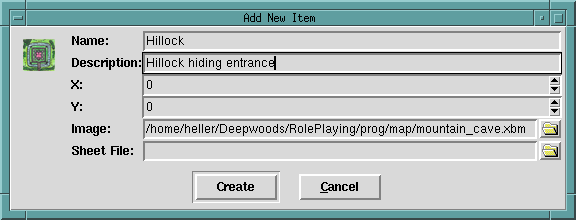
\includegraphics[width=5in]{CreatingHillock.png}
\caption{``Add New Item'' dialog box, adding the hillock hiding the entrance}
\label{fig:addnewitem}
\end{centering}
\end{figure}
\begin{figure}[hbpt]
\begin{centering}
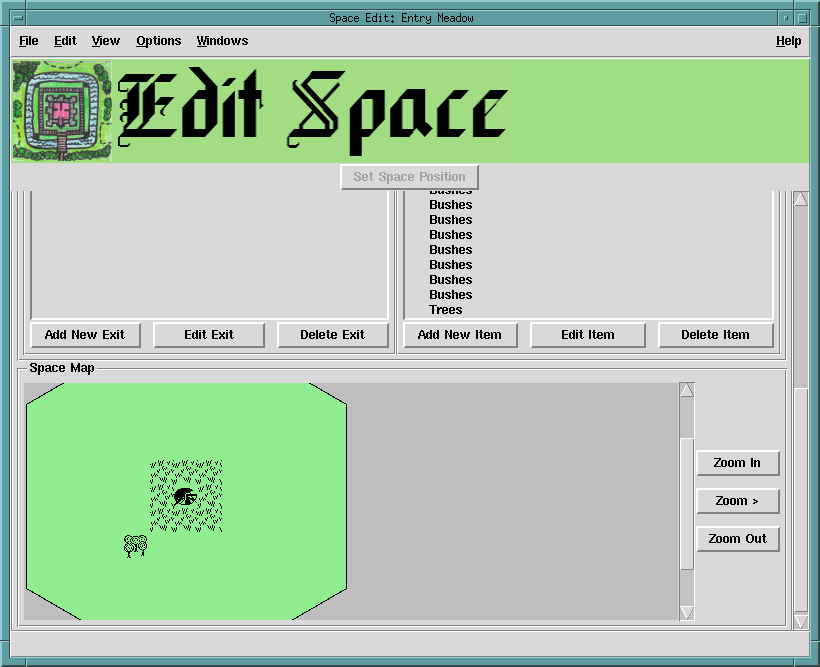
\includegraphics[width=5in]{UpdatedSpaceWithStairsHillockBushesTrees.png}
\caption{``Space Editor'' window for the ``Entrance Meadow'', after
adding the stairs, hollock, along with some bushes and trees}
\label{fig:entrymeadowspaceeditor2}
\end{centering}
\end{figure}
First we will add a set of spiral stairs leading down to the
strongholds first level.  We do this by clicking the ``Add New Exit''
button under the exit list.  A ``Add New Exit'' dialog box is
displayed.  After filling in the values we want, it looks like
Figure~\ref{fig:addnewexit}. Clicking ``Add'' adds this exit.  Next we
will add the hillock by clicking the ``Add New Item'' button under the
item list.  A ``Add New Item'' dialog box is displayed.  After filling
in the values we want, it looks like Figure~\ref{fig:addnewitem}. 
Clicking ``Add'' adds this item.  After adding some bushes and some
trees, the space map looks like
Figure~\ref{fig:entrymeadowspaceeditor2}\footnote{Since we added the
stairs and hillock at the same place, they are draw one over the
other.}\footnote{I used some elements from a collection of 24x24 X11
bitmaps I downloaded from Anthony Thyssen's icon collection at
\url{http://www.cit.gu.edu.au/~anthony/icons/}.}.



